\mode*
\section[Estado del arte]{Estado del arte}
\label{sec:arte}

\mode<presentation>{
  \begin{frame}[label=arte]
    \transduration{2}
    \frametitle{Cu\'al es el estado actual de la Caminata B\'ipeda?}
    \framesubtitle{Antecedentes y tendencias mundiales de investigaci\'on}
    \begin{center}
      \LARGE \textbf{\textcolor{blueun}{Estado del Arte}}
    \end{center}      
  \end{frame}
  \subsection[Investigaci\'on actual]{Algunas trabajos de investigaci\'on en la actualidad }
  \label{sec:algtra}
  \begin{frame}[label=timeline]
    \transduration{10}
    \frametitle{Breve historia de la rob\'otica b\'ipeda}
    \framesubtitle{Para entrar en contexto}
    \includegraphics[height=7.5cm,width=10.0cm]{../images/TimeLine05.png}
  \end{frame}
  \begin{frame}[label=tenencias]
    \transduration<1->{3}
    \frametitle{Trabajos relevantes de los \'ultimos 8 a\~nos}
    \framesubtitle{Tendencias mundiales en investigaci\'on}
    \begin{columns}[T]
      \begin{column}{2.0cm}
        \setbeamercovered{transparent}
        \uncover<2>{\includegraphics[height=7.5cm]{../images/TimeLineTendencias01.png}}
      \end{column}
      \begin{column}{5.0cm}
        \only<1>{
          \begin{center}
            \textbf{\textcolor{blueun}{Universidad de Waseda}}
            \begin{center}
              
\includegraphics[height=1.5cm]{../images/WasedaLogo.png}\\
            \end{center}
            \hspace{1.5cm}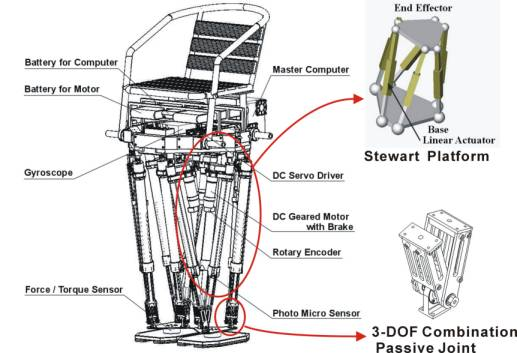
\includegraphics[height=3.8cm]{../images/WasedaTendencias.png}
          \end{center}
        }
        \only<2>{
          \begin{center}
            \textbf{\textcolor{blueun}{Honda Research Institute\\\& IHMC}}
            \begin{center}
              
\includegraphics[height=0.7cm]{../images/HondaLogo.png}\quad
              
\includegraphics[height=0.7cm]{../images/IHMCLogo.png}
            \end{center}
            \hspace{1.8cm}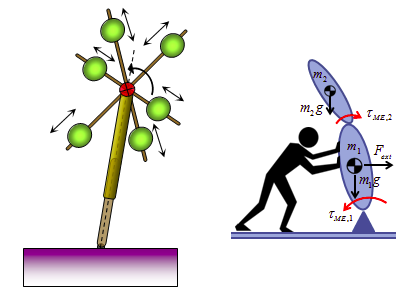
\includegraphics[height=4.0cm]{../images/HondaTendencias.png}            
          \end{center}
        }
        \only<3>{
          \begin{center}
            \textbf{\textcolor{blueun}{Aldebaran Robotics}}
            \begin{center}
              
\includegraphics[height=1.0cm]{../images/AldebaranLogo.png}\\
            \end{center}
            \vspace{0.5cm}\hspace{0.3cm}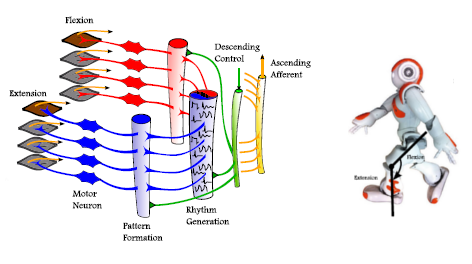
\includegraphics[height=4.0cm]{../images/AldebaranTendencias.png}            
          \end{center}
        }
        \only<4>{
          \begin{center}
            \textbf{\textcolor{blueun}{MIT\\Robot Locomotion Group}}\\
            \begin{center}
              
\includegraphics[height=1.0cm]{../images/MITLogo.png}
            \end{center}
            \vspace{0.5cm}\hspace{1.5cm}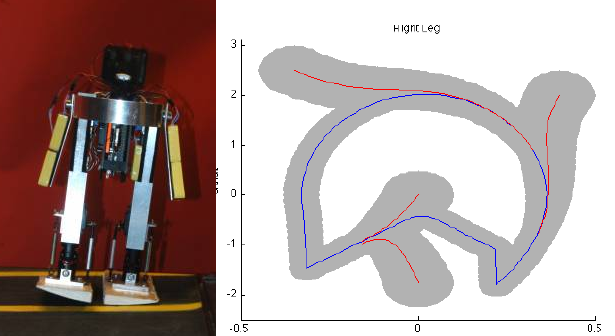
\includegraphics[height=3.0cm]{../images/MITTendencias.png}            
          \end{center}
        }
        \only<5>{
          \begin{center}
            \textbf{\textcolor{blueun}{ETH-BIRLab}}\\
            \begin{center}
              
\includegraphics[height=1.0cm]{../images/ETHLogo.png}
            \end{center}
          \vspace{0.5cm}\hspace{1.5cm}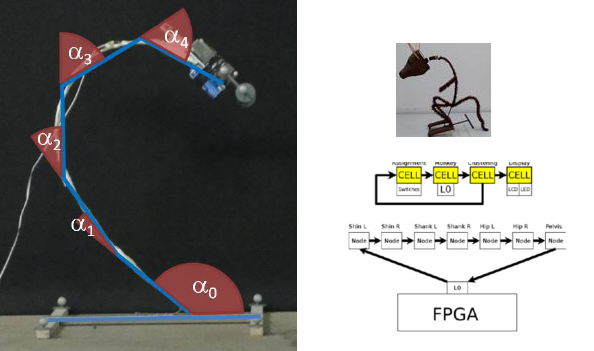
\includegraphics[height=4.0cm]{../images/ETHTendencias.png}
          \end{center}
        }
        \only<6>{
          \begin{center}
            \textbf{\textcolor{blueun}{CMU - Biorobotics and \\ CU - Locomotion Labs}}
            \begin{center}
              
\includegraphics[height=0.7cm]{../images/CMULogo.png}\\
              
\includegraphics[height=0.7cm]{../images/CornellULogo.png}
            \end{center}
            \vspace{0.1cm}\hspace{1.5cm}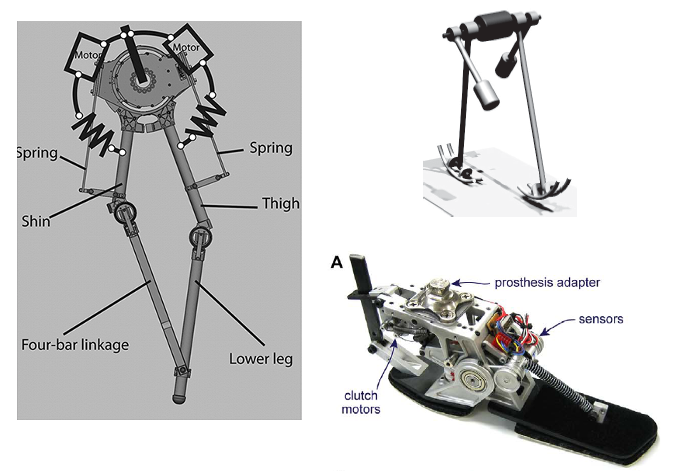
\includegraphics[height=3.5cm]{../images/CMUCornellTendencias.png}
          \end{center}
        }
        \only<7>{
          \begin{center}
            \textbf{\textcolor{blueun}{Delft University-DBL Lab}}\\
            \begin{center}
              
\includegraphics[height=1.0cm]{../images/DelftLogo.png}\\
            \end{center}
            \vspace{0.1cm}\hspace{2.5cm}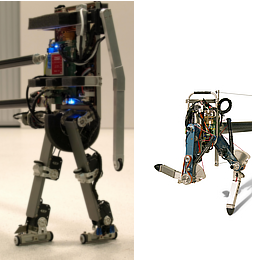
\includegraphics[height=4.0cm]{../images/DelftTendencias.png}
          \end{center}
        }
        \only<8>{
          \begin{center}
            \textbf{\textcolor{blueun}{Gottingen University}}
            \begin{center}
              
\includegraphics[height=1.5cm]{../images/GottingenULogo.png}
            \end{center}
            \vspace{0.1cm}\hspace{2.0cm}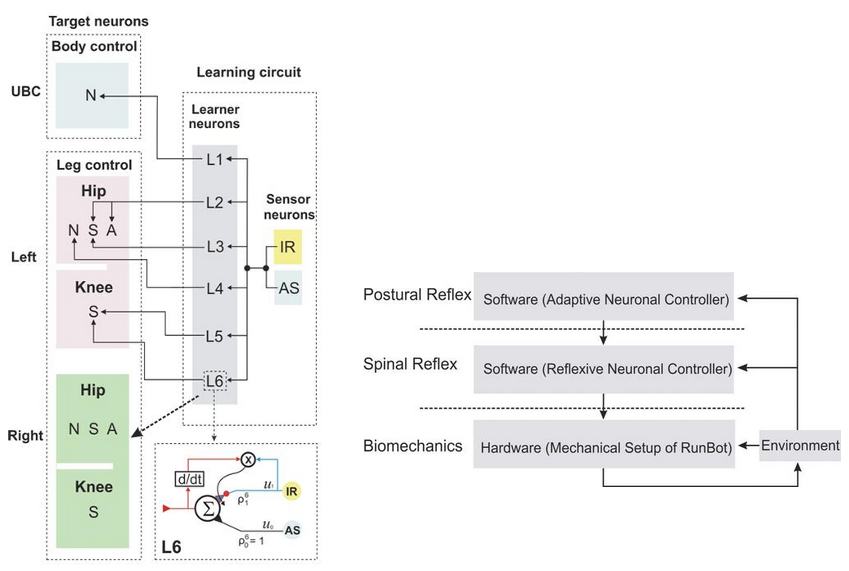
\includegraphics[height=3.5cm]{../images/GottingenUTendencias.png}
          \end{center}
        }
        \only<9>{
          \begin{center}
            \textbf{\textcolor{blueun}{CNRS}}
            \begin{center}
              
\includegraphics[height=2.0cm]{../images/CNRSLogo.png}\\
            \end{center}
            \vspace{0.1cm}\hspace{2.0cm}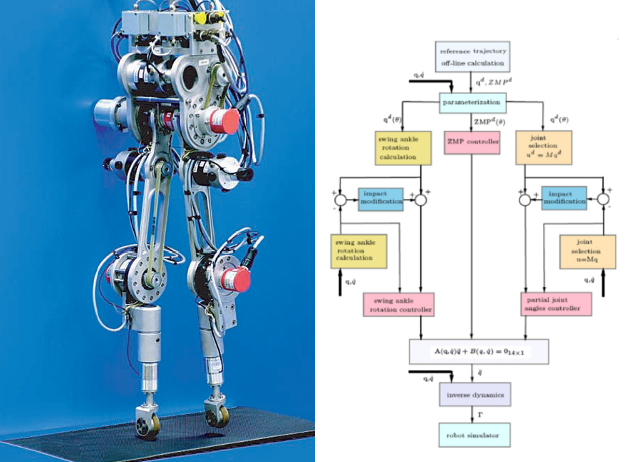
\includegraphics[height=3.5cm]{../images/CNRSTendencias.png}
          \end{center}
        }
        \only<10>{
          \begin{center}
            \textbf{\textcolor{blueun}{DLR-biped}}
            \begin{center}
              
\includegraphics[height=1.0cm]{../images/DLRLogo.png}\\
            \end{center}
            \vspace{0.1cm}\hspace{1.0cm}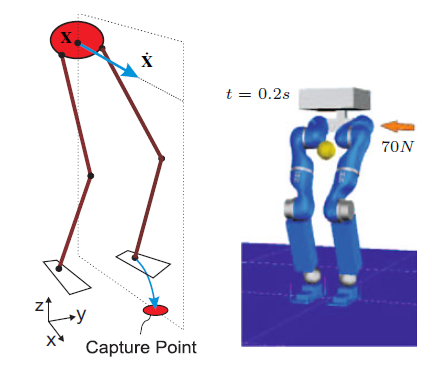
\includegraphics[height=4.0cm]{../images/DLRTendencias.png}
          \end{center}
        }
      \end{column}
      \begin{column}{3.5cm}
        \only<1>{
          \begin{center}
            \vspace{1.3cm}
            \textbf{\textcolor{blueun}{Tendencias}}
            \begin{itemize}\scriptsize
            \item Rob\'otica paralela
            \end{itemize}
            %\includegraphics[height=1.0cm]{../images/WasedaTendencias01.png}            
          \end{center}
        }
        \only<2>{
          \begin{center}
            \vspace{1.3cm}
            \textbf{\textcolor{blueun}{Tendencias}}
            \begin{itemize}\scriptsize
            \item Control
            \item Efectos del Torso
            \end{itemize}
          \end{center}
        }
        \only<3>{
          \begin{center}
            \vspace{1.3cm}
            \textbf{\textcolor{blueun}{Tendencias}}
            \begin{itemize}\scriptsize
            \item CPG, ANN
            \item AI, Aprendizaje
            \end{itemize}
          \end{center}
        }
        \only<4>{
          \begin{center}
            \vspace{1.3cm}
            \textbf{\textcolor{blueun}{Tendencias}}
            \begin{itemize}\scriptsize
            \item Control:{\tiny LQR-trees, SVM}
            \item Rob\'otica subactuada
            \end{itemize}
          \end{center}
        }
        \only<5>{
          \begin{center}
            \vspace{1.3cm}
            \textbf{\textcolor{blueun}{Tendencias}}
            \begin{itemize}\scriptsize
            \item Bajo costo
            \item CPG, SVM
            \item BAN
            \end{itemize}
          \end{center}
        }
        \only<6>{
          \begin{center}
            \vspace{1.3cm}
            \textbf{\textcolor{blueun}{Tendencias}}
            \begin{itemize}\scriptsize
            \item Balanceo, torso, SLIP
            \item Talon y tobillo
            \item Modelos Masa-resorte
            \end{itemize}
          \end{center}
        }
        \only<7>{
          \begin{center}
            \vspace{1.3cm}
            \textbf{\textcolor{blueun}{Tendencias}}
            \begin{itemize}\scriptsize
            \item Running robot
            \item Air Muscles and DC motors
            \item Balance
            \end{itemize}
          \end{center}
        }
        \only<8>{
          \begin{center}
            \vspace{1.3cm}
            \textbf{\textcolor{blueun}{Tendencias}}
            \begin{itemize}\scriptsize
            \item Aprendizaje de m\'aquina
            \item Control adaptativo
            \item Running Mode
            \end{itemize}
          \end{center}
        }
        \only<9>{
          \begin{center}
            \vspace{1.3cm}
            \textbf{\textcolor{blueun}{Tendencias}}
            \begin{itemize}\scriptsize
            \item Control y trayectoria
            \item Running Mode
            \end{itemize}
          \end{center}
        }
        \only<10>{
          \begin{center}
            \vspace{1.3cm}
            \textbf{\textcolor{blueun}{Tendencias}}
            \begin{itemize}\scriptsize
            \item Capture Points
            \item Control de torque de cuerpo completo
            \item Agarre de cuerpo completo
            \end{itemize}
          \end{center}
        }
      \end{column}
    \end{columns}
  \end{frame}
}
Revisando la amplia literatura encontrada sobre \emph{la locomoci\'on}, la mayor inquietud citada viene de la Rob\'otica\cite{Xiang2010,Mattar2013} y la Biomec\'anica\cite{Xiang2010,Mattar2013}, \'areas que muestran su interés en replicar las estructuras y/o las funcionalidades de movilidad de diferentes seres vivos\cite{Xu2013,Chiang2013} o como muchos autores\cite{Xu2013} y congresos\cite{RB2009} hacen referencia a \emph{biom\'imesis}. Estas necesidades van desde solo comprobar las leyes f\'isicas sobre un sistema mecatr\'onico\cite{Barker2010,Lens2011} hasta dise\~nar m\'aquinas robotizadas que sirvan al hombre en ambientes de riesgo donde \'este no deber\'ia encontrarse\cite{Seifried2014,Wu2013a}, o desde solo entender la marcha humana para proponer una terap\'ia sobre alg\'un m\'usculo lesionado\cite{Kang2013} hasta el remplazo de una extremidad que mejore la calidad de vida de una persona v\'ictima de alg\'un accidente\cite{Roa2006,Wu2013a}.\par
Dentro de la locomoci\'on b\'ipeda se diferencia dos formas generales del modo de andar: una bajo el r\'egimen de caminata y otra bajo el r\'egimen de correr, trotar o galopar\cite{Geyer2006}. La manera de distinguir estos modos viene dada por las distintas fase que definen un ciclo de andar, la diferencia entre caminar y trotar, ser\'a que durante la caminata habr\'an fases con doble contacto con el piso, mientras que en el r\'egimen de trotar o correr no existirá fases con doble contacto\cite{Geyer2006}, adem\'as en el regim\'en de correr existe una fase en la que no ocurre ningún contacto, fase que se encuentra con el nombre de vuelo.\par
Una de las posibles clasificaciones que se pude hacer en caminadores es seg\'un su tipo de balance durante la caminata, este balance puede ser est\'atico o din\'amico\cite{Braunl2008}. Las mayores inquietudes y retos al d\'ia de hoy se encuentran en el balance din\'amico, pues este tipo de balance se acerca m\'as a una caminata \'optima y natural, como la que han logrado los seres humanos durante toda su evoluci\'on.\par
Otra clasificaci\'on podr\'ia ser los modelos físico, que se han utilizado para describir la caminata\cite{Xiang2010}: 1) modelos de p\'endulo invertido, 2) din\'amica pasiva de la caminata y 3) ZMP punto de momento cero. Una caracter\'istica de los tres modelos f\'isico citados anteriormente, es que sus movimientos son generados en tiempo real\cite{Xiang2010}. En el caso de la din\'amica pasiva de la caminata, recientes tendencias en b\'usqueda de dise\~nos naturales tanto en las estructuras mec\'anicas como en los esquemas de control buscan mejorar los problemas energ\'eticos que resultaron de los mejores avances que se han obtenido en el tema gracias al concepto del ZMP\cite{Xiang2010}.\par
Aunque la caminata pasiva lleva en estudio m\'as de 25 a\~nos, tuvo un momento de oscuridad cuando el ZMP, el cual lleva m\'as de 40 a\~nos, logr\'o resultados tecnol\'ogicos en los a\~nos ochenta\cite{Vukobratovic2004}. Desde hace 25 a\~nos se retomo nuevamente el estudio de la caminata pasiva ya no solo como ejemplo acad\'emico\cite{McGeer1990a}, dando nuevos caminos en el control y acerc\'andose a la soluci\'on desde el punto de vista de la optimizaci\'on de la energ\'ia\cite{Goswami1996}, proponiendo as\'i a la caminata activa la generaci\'on \'optima de trayectorias\cite{Gregg2010}.\par
Los modelo mec\'anicos bio-inspirados se encuentran de dos clases\cite{Xiang2010}. El primero que toma el sistema \'oseo para luego proponer unos actuadores distintos a los músculos\cite{Wang2012} y el segundo que analiza adem\'as del sistema \'oseo, el sistema muscular para tomar los m\'usculos del cuerpo humano como los actuadores del sistema\cite{Kang2013,Roa2006}. Los modelos matem\'aticos de estos modelos bio-inspirados est\'an basados en la din\'amica multicuerpo\cite{Xiang2010}, donde cabe resaltar que los modelos m\'usculo-esquel\'eticos incrementan la carga computacional por el gran n\'umero de grados de libertad\cite{Xiang2010}, mientras que los modelos basados \'unicamente en el sistema oseo son f\'aciles de simplificar y en la mayor\'ia de los casos tan solo se tiene en cuenta las longitudes de las extremidades analizadas reduciendo también un importante n\'umero de grados de libertad\cite{McGeer1990a}. Cabe resaltar de diferentes herramientas y formalismos son empleadas en la literatura para la generaci\'on de modelos, en donde se encuentran: Newton-Euler, Euler-Lagrange, Hamilton, Kane, \'algebras especiales para entender el espacio tridimensional como los Screws y los cuaterniones o el método de Denavit-Hartenverg y finalmente la conservaci\'on del momento angular para representar las colisiones de los sistemas.\par
Dentro del problema de la din\'amica multicuerpo, se enfrentan dos pilares, 1) la din\'amica inversa, donde las trayectorias se conocen en un comienzo o se pueden tomar arbitrarias para luego encontrar las cargas requeridas por los actuadores y 2) la din\'amica directa en donde se conocen las cargas en los actuadores, y resolviendo un sistema de ecuaciones diferenciales con condiciones iniciales de segundo orden se puede encontrar la evoluci\'on temporal de las articulaciones en el espacio.\par
Una vez se logra un modelo f\'isico del caminador, surgen los problemas de generaci\'on de las trayectorias. La generaci\'on de trayectorias es un problema abierto que se aborda con muchas t\'ecnicas y seg\'un los objetivos de la investigaci\'on\cite{Kherici2014,Mahmoodabadi2014}. Una clasificaci\'on dada por\cite{Xiang2010}, divide la generaci\'on de trayectorias en m\'etodos basados en optimizaci\'on y m\'etodos basados en control. Ambos son lo suficientemente costos para ser implementados en tiempo real sin exagerar los recursos de c\'omputo\cite{Mahmoodabadi2014}. Adem\'as de esto es com\'un emplear los m\'etodos de optimizaci\'on y control en conjunto para encontrar la soluci\'on.\par
Las dificultades presentes en la generaci\'on de trayectorias tienen 1) la complejidad computacional de la programaci\'on no-lineal adem\'as de una optimizaci\'on multiobjetivo, en la que se pueden encontrar restricciones de diferentes clases\cite{Mahmoodabadi2014}, 2) los modelos h\'ibridos presentes en los modelos de mec\'anica multicuerpo introducen discontinuidades en las funciones objetivo, lo que propone que los m\'etodos de b\'usqueda basados gradiente sean descartados\cite{Xiang2010}, tambi\'en se proponer mediciones del rendimiento de la marcha que eviten dichas discontinuidades para usar los m\'etodos de b\'usqueda basados en gradiente\cite{Xiang2010}.\par
Dependiendo como se aborde el problema de la din\'amica, inverso o directo, es posible que la generaci\'on de las trayectorias implique, la soluci\'on de las ecuaciones diferenciales, este es el caso de la d\'inamica directa en el que se proponen las cargas sobre el sistema pero se desconocen las trayectorias, es ac\'a cuando la variable de dise\~no en este caso las cargas, se deben buscar la mejor evoluci\'on de cargas en el tiempo, que satisfaga las condiciones de dise\~no.\par

\subsection[Estado del arte UN]{Estado del arte en al Universidad Nacional de Colombia}
\label{sec:estadoUN}
\mode<presentation>{
  \begin{frame}[label=tendenciasUN]
    \transduration<1->{2}
    \frametitle{Cual es la actualidad y antecedentes en la UN?}
    \framesubtitle{Robotica b\'ipeda y temas afines desarrollados en la UN}
    \begin{columns}[T]
      \begin{column}{6cm}
        \setbeamercovered{transparent}
        Descripci\'on serie UNROCA:
        \begin{enumerate}\scriptsize
        \item<2-> Modelo PWD con rodillas
        \item<3-> Ciclos L\'imite
        \item<4-> Bifurcaciones y caos
        \item<5-> Metodolog\'ia de dise\~no
        \item<6-> UNROCA-I
        \item<7-> UNROCA-II
        \item<8-> UNROCA-III
        \end{enumerate}
        \visible<9->{\uncover<9->{
        Temas relacionados:
        \begin{enumerate}\scriptsize
        \item<10-> Rob\'otica subactuada
        \item<11-> Caminata animal b\'ipeda
        \end{enumerate}}}
      \end{column}
      \begin{column}{4cm}
        \vspace{-0.5cm}
        \only<1>{
          \begin{center}
            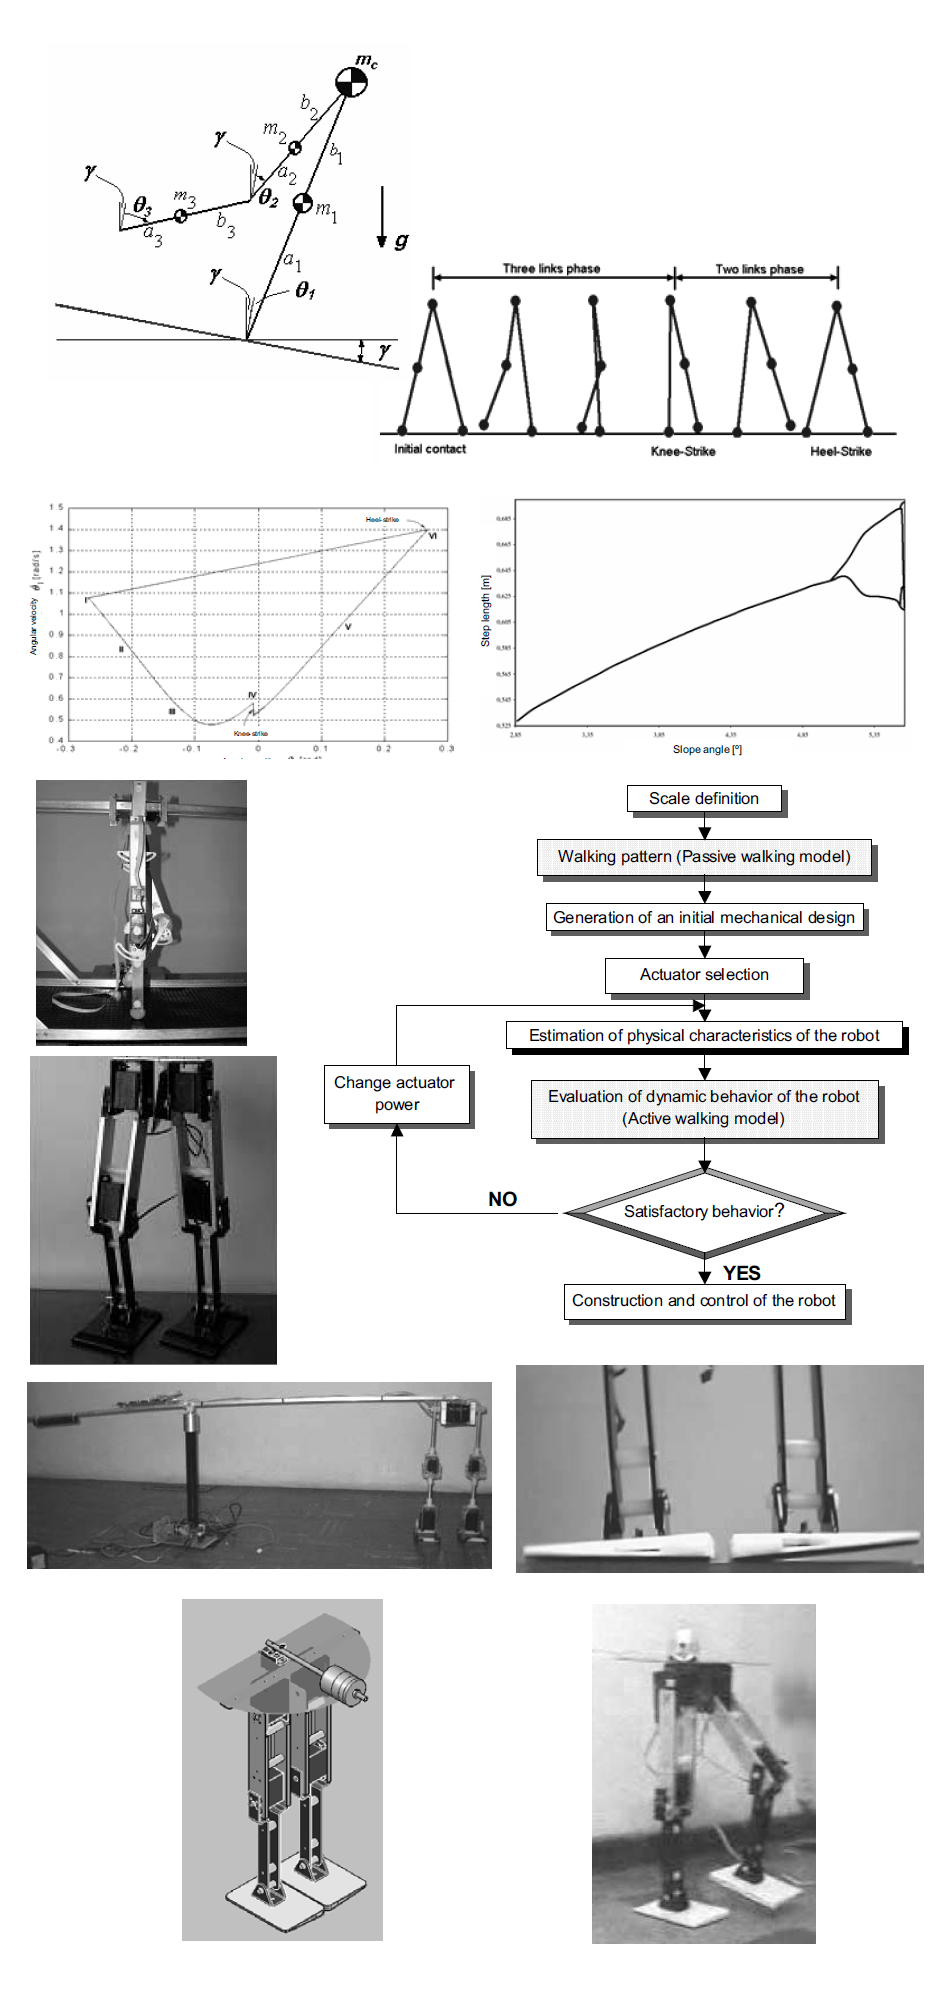
\includegraphics[height=7cm]{../images/UNROCA.png}
          \end{center}
        }
        \only<2>{
          \begin{center}
            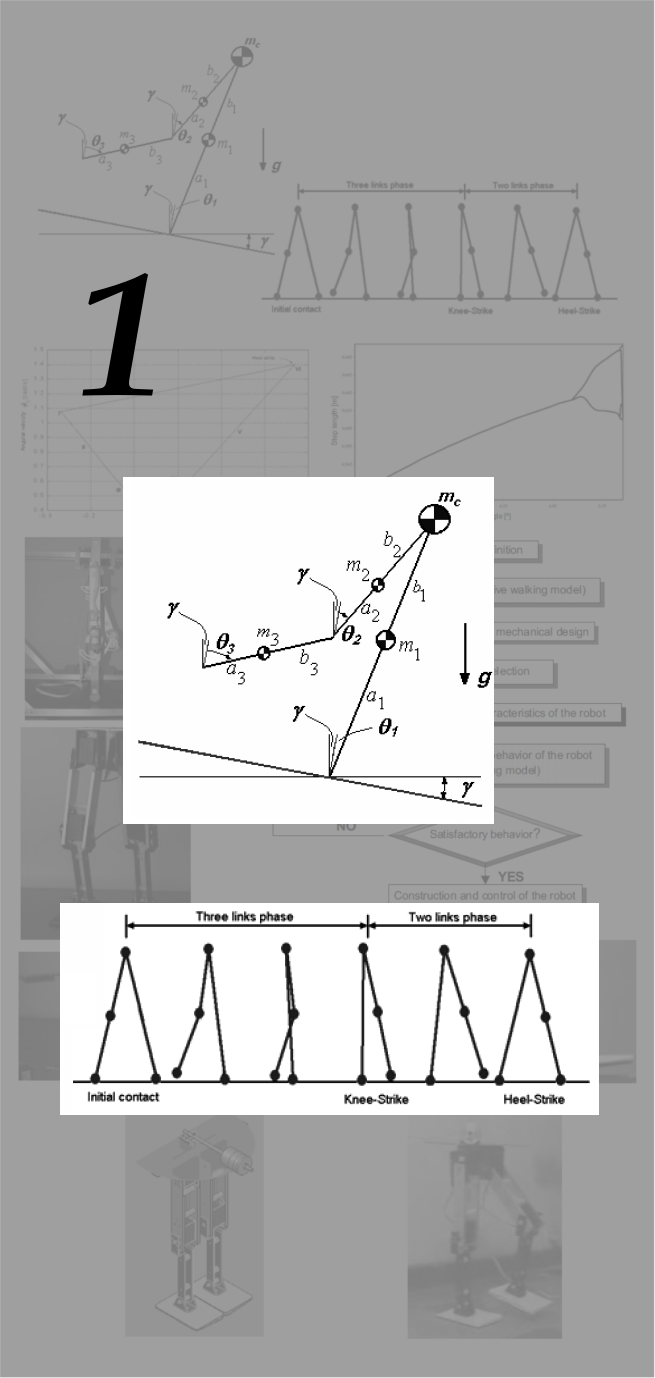
\includegraphics[height=7cm]{../images/UNROCA_0.png}
          \end{center}
        }
        \only<3>{
          \begin{center}
            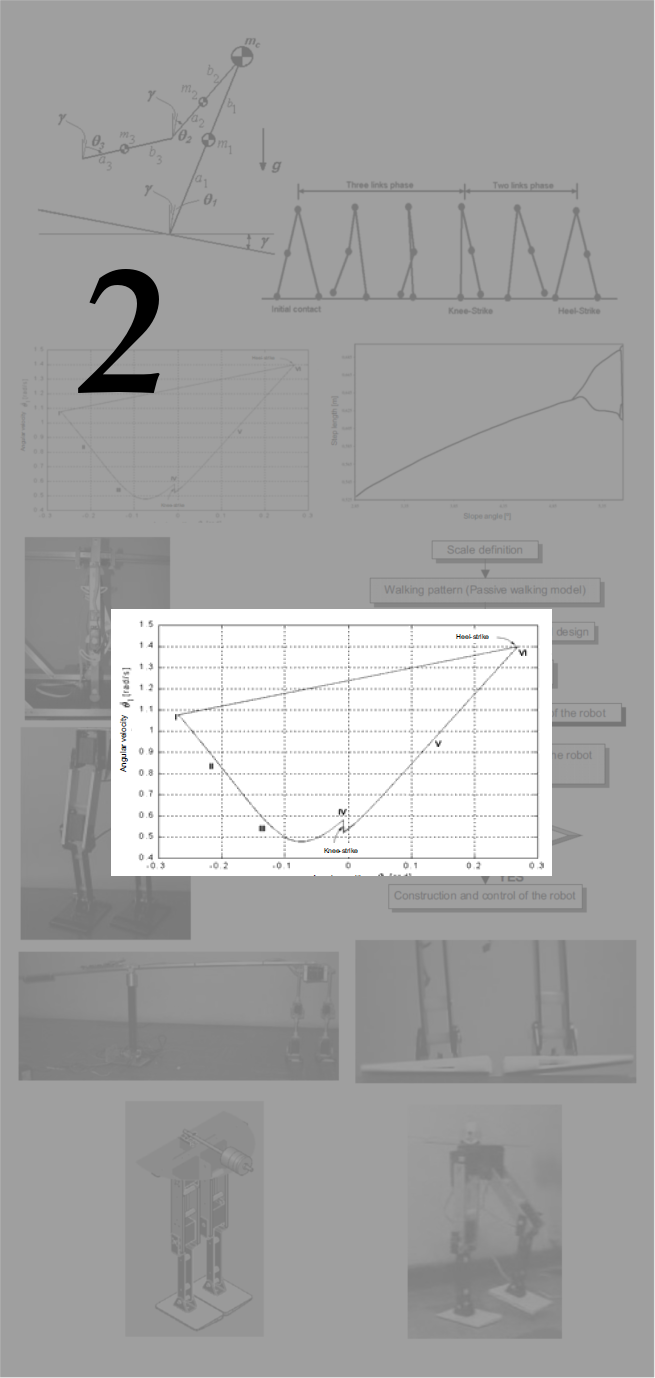
\includegraphics[height=7cm]{../images/UNROCA_1.png}
          \end{center}
        }
        \only<4>{
          \begin{center}
            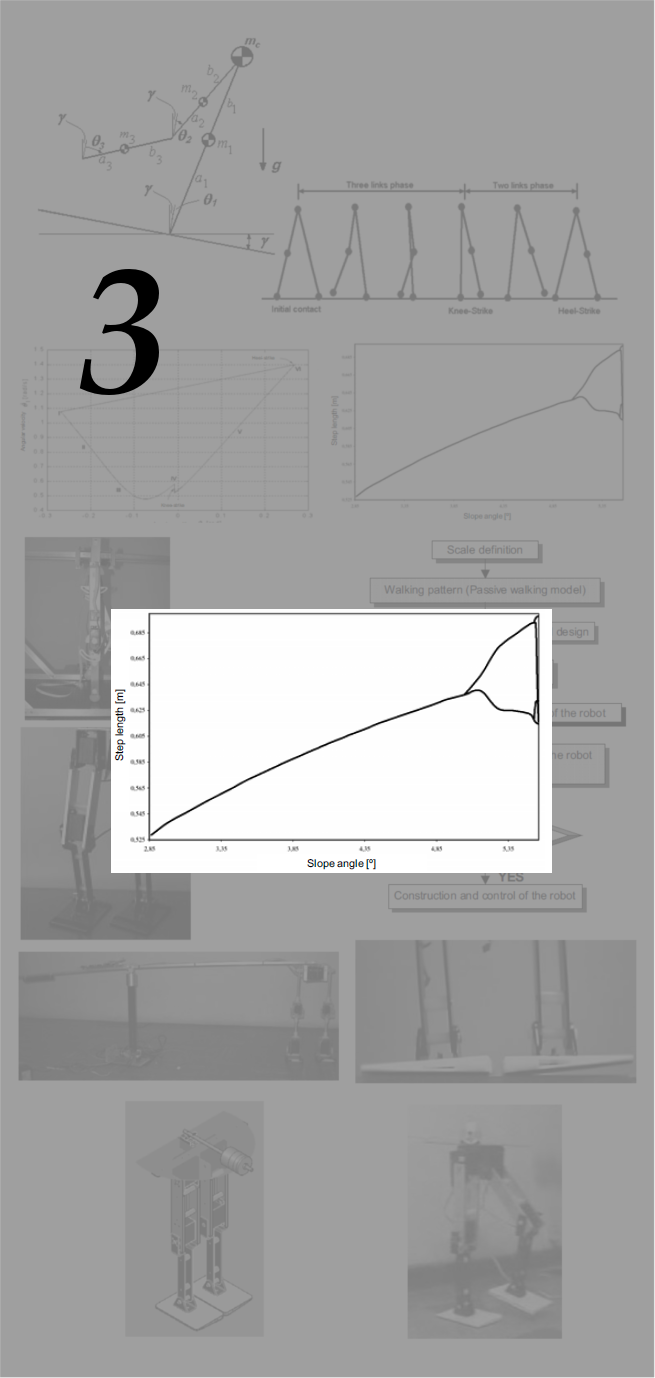
\includegraphics[height=7cm]{../images/UNROCA_2.png}
          \end{center}
        }
        \only<5>{
          \begin{center}
            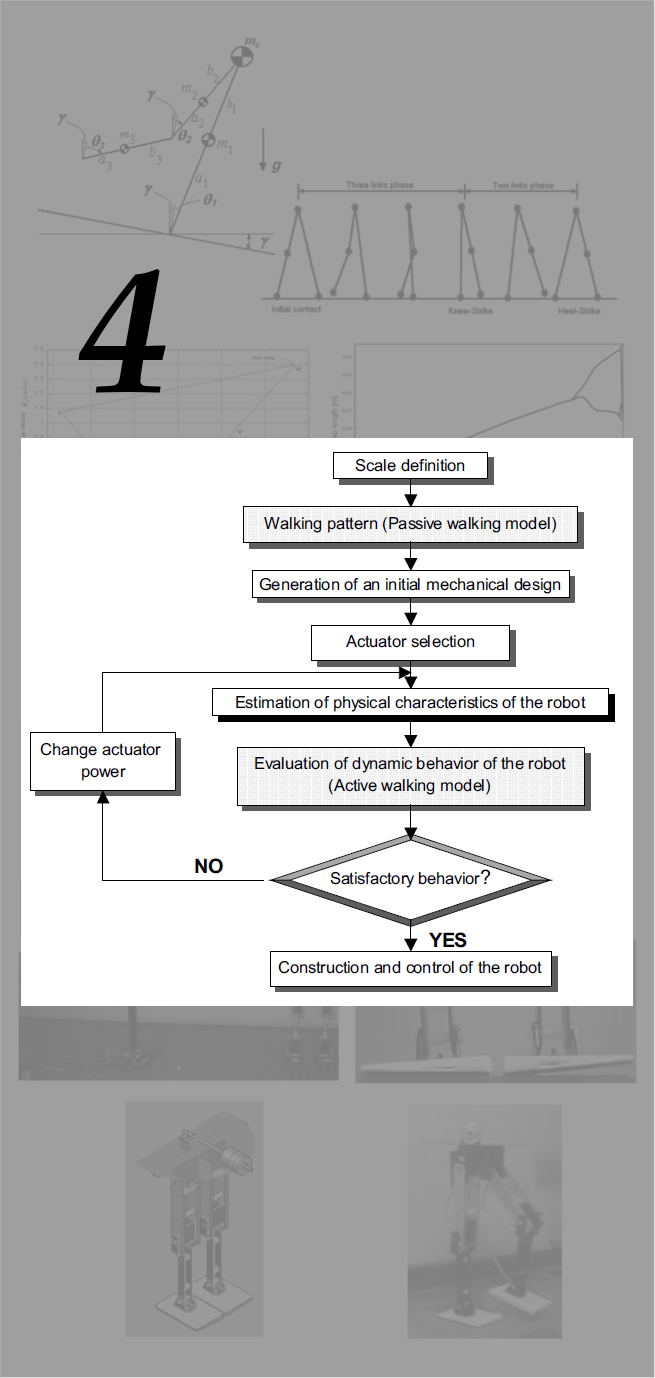
\includegraphics[height=7cm]{../images/UNROCA_3.png}
          \end{center}
        }
        \only<6>{
          \begin{center}
            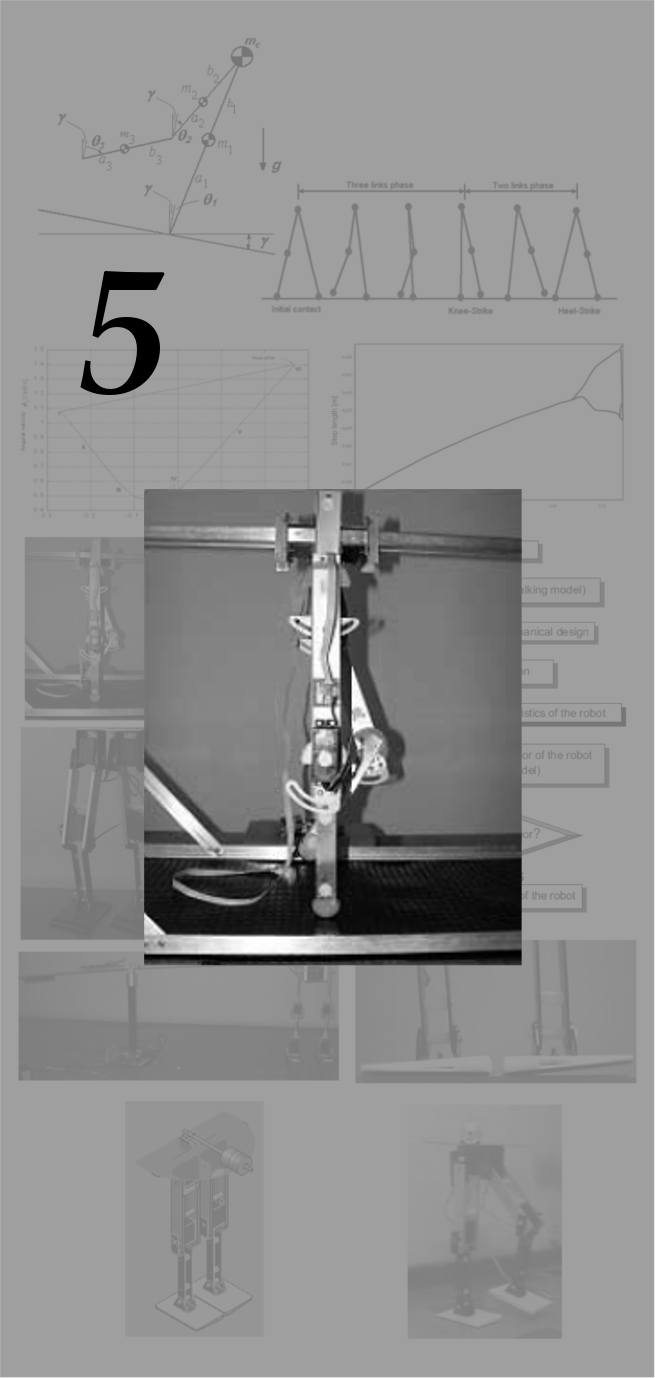
\includegraphics[height=7cm]{../images/UNROCA_4.png}
          \end{center}
        }
        \only<7>{
          \begin{center}
            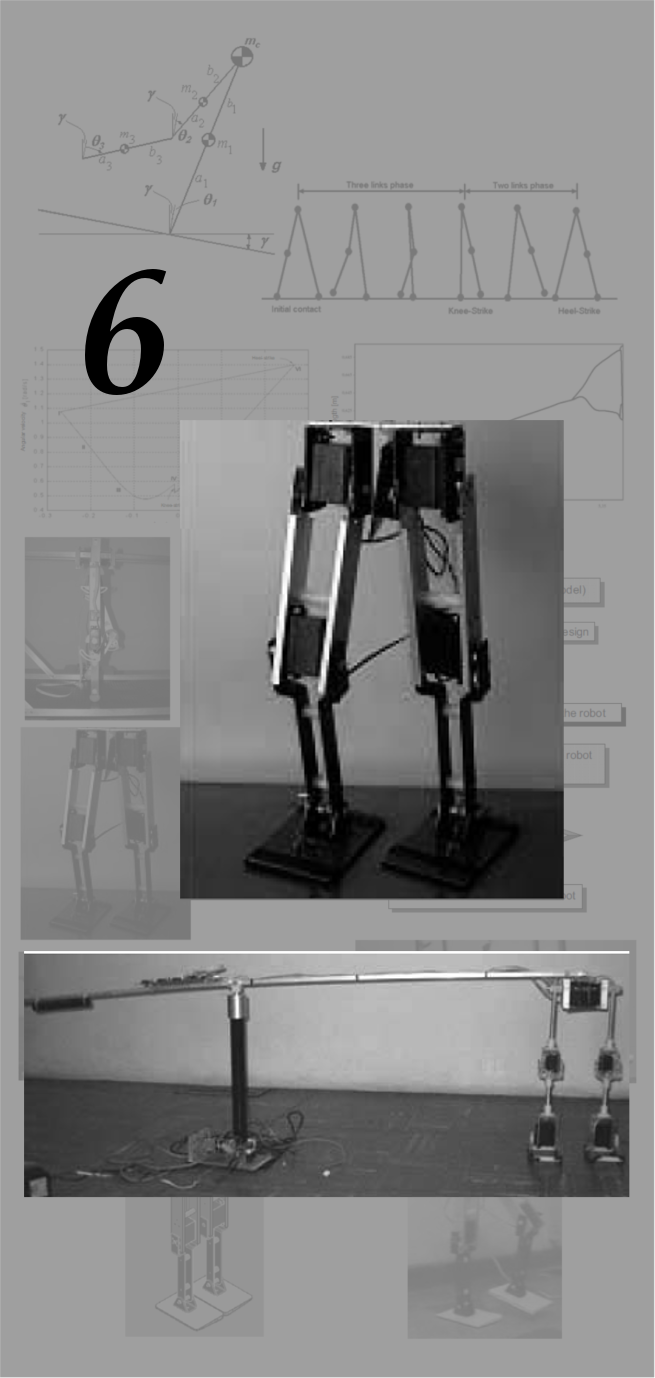
\includegraphics[height=7cm]{../images/UNROCA_5.png}
          \end{center}
        }
        \only<8>{
          \begin{center}
            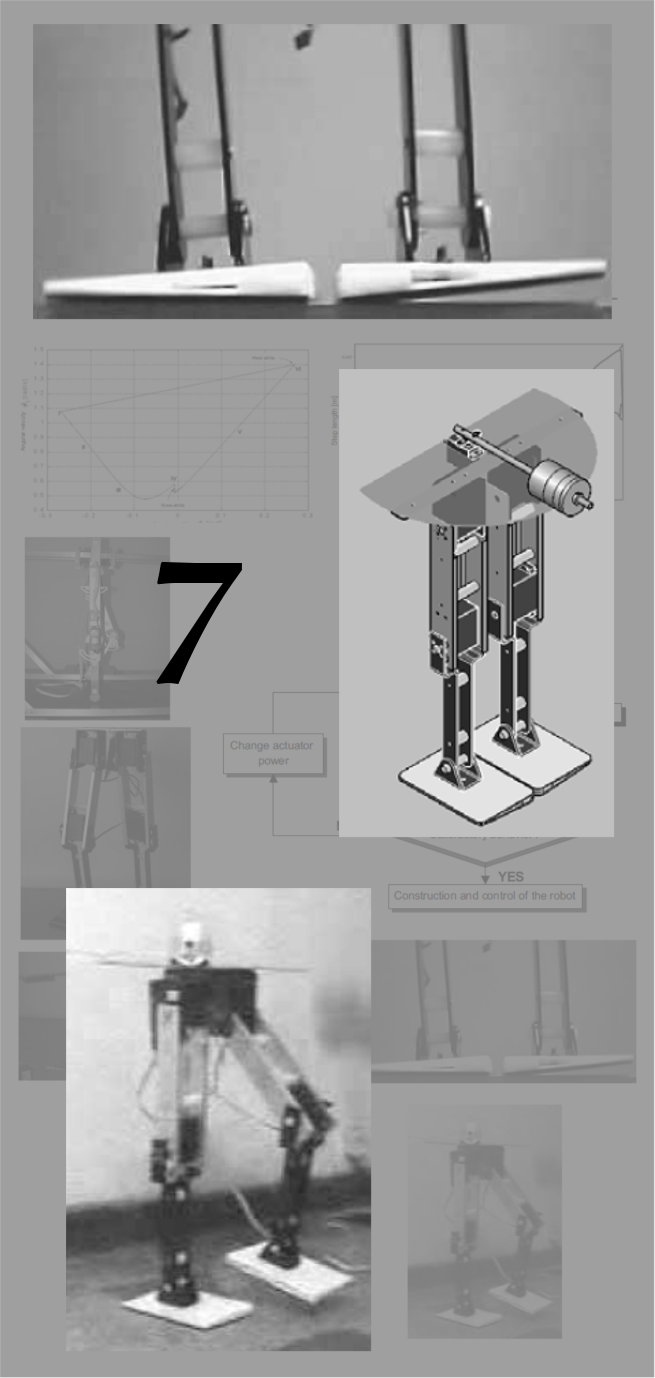
\includegraphics[height=7cm]{../images/UNROCA_6.png}
          \end{center}
        }
        \only<9-10>{
          \begin{center}
            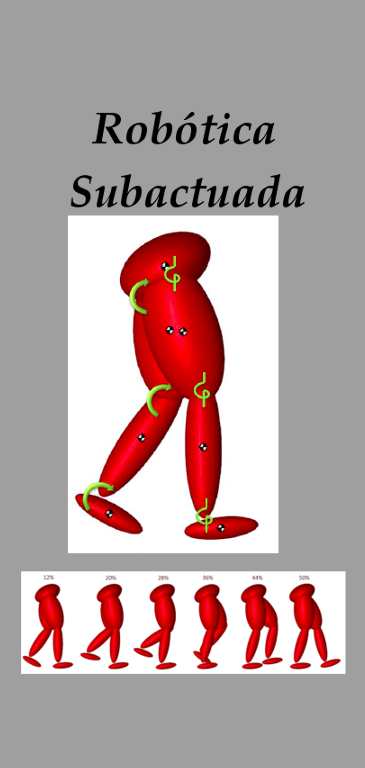
\includegraphics[height=7cm]{../images/UNRSubactuada.png}
          \end{center}
        }
        \only<11>{
          \begin{center}
            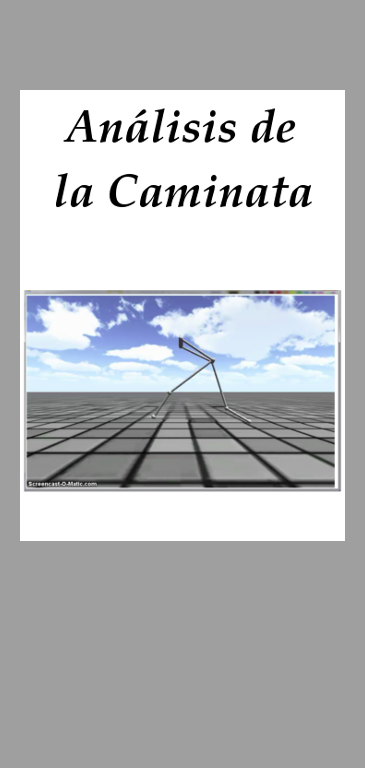
\includegraphics[height=7cm]{../images/UNACaminata.png}
          \end{center}
        }
      \end{column}
    \end{columns}
  \end{frame}
  \subsection[Resumen]{Resumen de tendencias }
  \label{sec:resten}
  \begin{frame}[label=resumen]
    \transduration<1-7>{0.8}
    \frametitle{Hacia una framework de rob\'otica b\'ipeda}
    \framesubtitle{Resumen de tendencias por \'area en Rob\'otica B\'ipeda}
    \begin{center}
      \only<1-7>{
        \vspace{-2.2cm}
        \begin{columns}[c]
          \begin{column}{3cm}
            \only<1,3-6>{\setbeamercolor{postit}{fg=white,bg=red!40!black}}
            \only<2,7>{\setbeamercolor{postit}{fg=white,bg=red}}
            \begin{beamercolorbox}[sep=0.5em,wd=3cm,rounded=true,center,shadow=true]{postit}
              \begin{enumerate}\tiny
              \item CAN-bus
              \item WSN
              \item BAN
              \item GNU/Linux-Embedded
              \end{enumerate}
              \textbf{Sistemas Embebidos}
            \end{beamercolorbox}
          \end{column}
          \begin{column}{3cm}
            \only<1-2,4-6>{\setbeamercolor{postit}{fg=white,bg=yellow!60!black}}
            \only<3,7>{\setbeamercolor{postit}{fg=white,bg=yellow}}
            \begin{beamercolorbox}[sep=0.5em,wd=3cm,rounded=true,center,shadow=true]{postit}
              \begin{enumerate}\tiny
              \item An\'alisis de marcha
              \item Pr\'otesis y asistencia
              \item Mod. de articulaciones
              \item Tal\'on-Planta-Antepi\'e
              \end{enumerate}
              \textbf{Biomec\'anica}
            \end{beamercolorbox}
          \end{column}
          \begin{column}{3cm}
            \only<1-3,5-6>{\setbeamercolor{postit}{fg=white,bg=blue!40!black}}
            \only<4,7>{\setbeamercolor{postit}{fg=white,bg=blue}}
            \begin{beamercolorbox}[sep=0.5em,wd=3cm,rounded=true,center,shadow=true]{postit}
              \begin{enumerate}\tiny
              \item An\'alisis y s\'intesis
              \item Efi. energ\'etica(ej.SLIP)
              \item Efe.de Torso y Balance
              \item Rob\'otica Paralela
              \end{enumerate}
              \textbf{Modelado y Mecanismos}
            \end{beamercolorbox}
          \end{column}
        \end{columns}
        \vspace{1.0cm}
        \begin{columns}[c]
          \begin{column}{3cm}
            \only<1-4,6>{\setbeamercolor{postit}{fg=white,bg=black}}
            \only<5,7>{\setbeamercolor{postit}{fg=white,bg=white!50!black}}
            \begin{beamercolorbox}[sep=0.5em,wd=3cm,rounded=true,center,shadow=true]{postit}
              \textbf{C. Flexible y Optimizaci\'on}
              \begin{enumerate}\tiny
              \item Optim. Topol\'ogica
              \item GA's, PSO
              \item Fuzzy,ANN,CPG,SVM
              \item Agentes inteligentes
              \end{enumerate}
            \end{beamercolorbox}
          \end{column}
          \begin{column}{3cm}
            \only<1-5>{\setbeamercolor{postit}{fg=white,bg=green!40!black}}
            \only<6,7>{\setbeamercolor{postit}{fg=white,bg=green}}
            \begin{beamercolorbox}[sep=0.5em,wd=3cm,rounded=true,center,shadow=true]{postit}
              \textbf{Control y Sis. Din\'amicos}
              \begin{enumerate}\tiny
              \item Map. Poincare
              \item Control \'Optimo LQR
              \item Contorl Adaptativo
              \item Control de torque
              \end{enumerate}
            \end{beamercolorbox}
          \end{column}
        \end{columns}
        \vspace{-4.6cm}
        \hspace{-0.25cm}
        \setbeamercolor{postit}{fg=white,bg=blueun}
        \begin{beamercolorbox}[sep=0.5em,wd=4.0cm,rounded=true,center]{postit}
          \textbf{\Large\textcolor{white}{ROB\'OTICA B\'IPEDA}}
        \end{beamercolorbox}
      }
    \end{center}
  \end{frame}
}
El departamento de Ingenier\'ia Mec\'anica y Mecatr\'onica hacia 2003, bajo los grupos de investigaci\'on de Biomec\'anica y Robots M\'oviles, construye tres modelos de caminadores, en donde las patrones de marcha son generados por el an\'alisis y simulaci\'on de caminadores pasivos y posteriormente las trayectorias de las articulaciones son reproducidas por los caminadores activos construidos. Adicionalmente se propone una metodolog\'ia de dise\~no\cite{Heredia2007}.\par
El modelo de tres eslabones y cuatro masas puntales cl\'asico estudiado antes por\cite{McGeer1990a}, se obtienen distintas trayectorias de los \'angulos de las articulaciones para diferentes velocidades de marcha que son directamente relacionadas con las pendientes de inclinaci\'on del piso\cite{M2005}, es importante mencionar que se incluye un an\'alisis adimensional de parámetros y un an\'alisis de las propiedades ca\'oticas del caminador bípedo analizado\cite{M2005a}. Los datos obtenidos en la fase anterior, son convertidos a los requeridos por la construcci\'on f\'isica implementada.\par
A continuaci\'on se muestran los tres robot UNROCA generados en el departamento Figura.\ref{fig:unroca}, los dos primeros intentos mostraban la reproducci\'on de las trayectorias generadas en la primera fase, pero usaban soportes estructurales para alcanzar la estabilidad. En el tercer intento el robot aseguro su estabilidad con el uso de una masa oscilante a la altura de la cadera, se incorporan granes pies para la estabilidad est\'atica. Bajo el r\'egimen de marcha la estabilidad es asegurada en acci\'on del contrapeso oscilante y el criterio de ZMP de la trayectoria previamente calculada. La trayectoria es seguida usando controles PD y utilizando servomotores. Por cada par de servos es utilizado un microcontrolador m\'as un microcontrolador central\cite{M2005}.
\begin{figure}[!hbt]
  \centering
  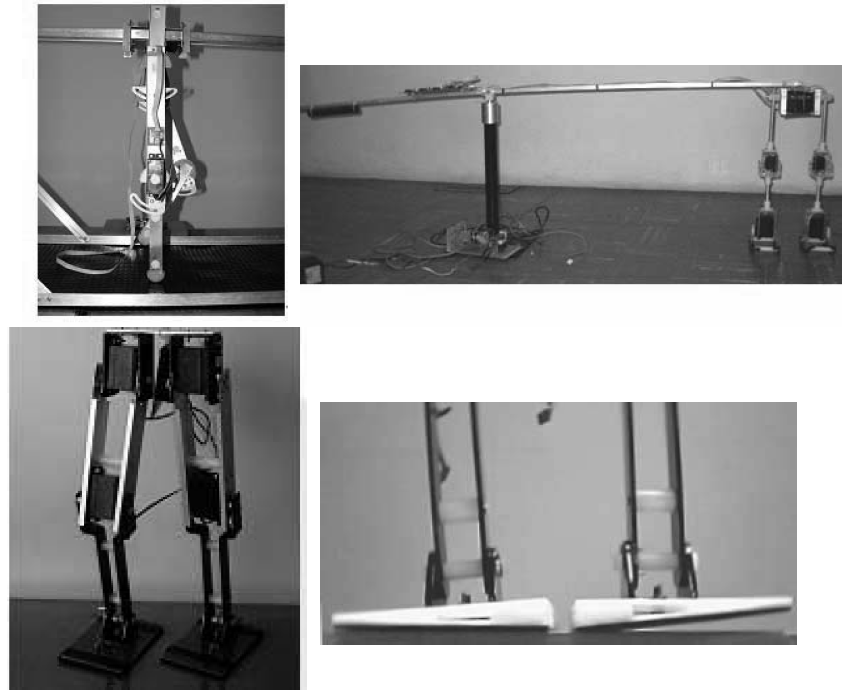
\includegraphics[scale=0.4]{../images/unroca.png}
  \caption{Robots serie UNROCA. [Tomado de \cite{M2005}]}
  \label{fig:unroca}
\end{figure}

\mode<article>{
  \subsection[Investigaci\'on actual]{Algunas trabajos de investigaci\'on en la actualidad }
  \label{sec:algtra}

  \subsubsection[Gen. Tray. y Control]{Generaci\'on de trayectorias y control}
  \label{sec:gentray}
  Simulaci\'on de un robot b\'ipedo empleando una m\'etodo evolutivo. 10 DOF y 7 eslabones, el m\'etodo PSO (Particle swarm optimization) asegura la estabilidad usando como restricci\'on el centro de masa CoM del pol\'igono de soporte\cite{Kherici2014}.\par
  Se compara varios m\'etodos de optimizaci\'on multiobjetivo NSGAII, Sigma method, MOGA con el m\'etodo MOPSO. El m\'etodo es utilizado para sintonizar un controlador "robust sliding tracking". En el proceso se reduce una b\'usqueda heur\'istica de parámetros por ensayo-error, a una b\'usqueda \'optima seg\'un criterios de dise\'~no. Un operador de turbulencia es utilizado para evadir \'optimos locales\cite{Mahmoodabadi2014}.\par
  Se proponen trayectorias \'optimas y din\'amicamente estables para subir y bajar escaleras basadas en el movimiento humano. Siete caracter\'isticas son resaltadas. Un algoritmo gen\'etico de c\'odigo real es utilizado para optimizar la marcha del robot y mejorar el consumo de energ\'ia y fortalecer la estabilidad. Simulaciones sobre configuraciones de 12-DOF son simuladas, basadas en las capturadas del movimiento humano durante el ascenso y el descenso de escaleras\cite{Lim2014}.\par
  Se emplea un control (0-flat normal form) en una plataforma b\'ipeda de 7-DOF. Los resultados obtenidos muestran el buen desempe\~no de este m\'etodo para proponer leyes de control en sistemas altamente no-lineales. Adicional se propone una estrategia de dise\~no para controladores en robots caminadores\cite{Bououden2014}.\par
  Se plantea un control compensado para evitar que perturbaciones externas, saquen de control el sistema. El sistema de aprendizaje mediante m\'aquinas de soporte vectorial difuso. Los resultados son comparados con otros m\'etodos inteligentes y se muestra su superioridad, mostrando una mayor sensibilidad y aumentando los rangos de estabilidad. En las fases de SSP y DSP se introducen conjunto de pertenencia de  triangulares y Gauss que permiten formular propiedades temporales de las marchas de robots con perturbaciones externas\cite{Wang2013}.\par
  Usando el robot ePaddle, dise\~nado para actuar en medios terrestres, acu\'aticos y terrenos anfibios. Se estudia la marcha en modo carrera caminata. Simulaciones subiendo escaleras y siguiendo trayectorias circulares, muestran la estabilidad y eficiencia encontrada\cite{Sun2013}.\par
  Generaci\'on en tiempo real de trayectorias para un robot de siete eslabones planar\cite{Farzaneh2014}.\par

  \subsubsection[Bioinspiardos y mecanismos]{Biomec\'anica, Caminata,  Modelado y S\'intesis de mecanismos}
  \label{sec:ascapa}
  Un arreglo de sensores de fuerza flexible (FFSA) es construido para caracterizar el contacto del pie con terrenos irregulares, para determinar el área efectiva de contacto (ECA). Esta área es importante para mantener el balance dinámico y por lo tanto es utilizado en un esquema adicional de control para caminar sobre terrenos irregulares\cite{Wu2013}.\par
  Una rodilla basada en mecanismos de cuatro barras es investigada en el desempe\~no de robots bípedos. Es comparada con la articulaci\'on tradicional rotacional de los robots. Concluyendo que aunque para bajas velocidades la articulaci\'on rotacional es mejor, en altas velocidades el mecanismo de cuatro barras muestra un mejor desempe\~no. El mecanismo de cuatro barras es optimizado siguiendo los ciclos de marcha óptimos\cite{Aoustin2013}.\par
  Se dise\~na una rodilla (mediante optimizaci\'on perimétrica) basada en rodadura natural de la rodilla, se obtiene un mejoramiento en el consumo energético de los actuadores comparados con las rodillas de rotación tradicional\cite{Hobon2014}.\par
  Modelado del efecto del contacto de rodadura de la planta del pie en la dinámica de caminar. El contacto es descrito por las longitudes del retropie, mediopie y antepie. Los parámetros anteriores son relacionado con los principales descriptores de marcha como la velocidad media , el periodo de paso en ángulo de entrepierna y la longitud de paso, así como la energía mecánica. Estas relaciones resultan útiles para el dise\~no de prótesis y la estabilidad del sistema\cite{Mahmoodi2013}.\par
  Un nuevo dise\~no m\'as parecido a las características humanas en cuanto a la rodilla, el contacto de la planta del pie, inspirados en la forma del esqueleto humano, especialmente la pelvis. Las ventajas de la pelvis se ven reflejadas en el manejo del centro de gravedad de la parte superior del cuerpo humano. Un mejor modelo del pie conlleva a modelo de péndulo invertido durante sus fases\cite{Chiang2013}.\par
  Basados en el modelo de la din\'amica de la caminata pasiva, específicamente la marcha del compás, la cual exhibe propiedades de caos. Se linealiza el modelo alrededor de un ciclo limite híbrido. Usando los mapas de Poincar\'e, es dise\~na un control por realimentaci\'on de estados, para convertir el sistema pasivo en activo\cite{Gritli2013}.\par
  Se realiza el dise\~no de la lagartija Jesucristo, basado en un mecanismos Watt-I y los grupos de Assur. Se utiliza un algoritmo de control CPG(Central Pattern Generator) del sistema neural, para el balance y el ajusta de la marcha \cite{Xu2013}.\par
  Análisis del modelo dinámico, estabilidad y consumo de energ\'ia eficiente de un robot con seis extremidades\cite{Roy2013}.\par
}